%DEMONSTRATION FILE FOR eACCESSIBILITY - VERSION 29 JULY 2020
\documentclass[12pt]{article}
\usepackage{latexsym,graphicx,color}
\usepackage{amssymb,amsmath,amsfonts}
\usepackage{lscape}
%
\title{Towards fully eAccessible documents}
\author{Sam Fearn and Anne Taormina}

%Improved Accessibility - uncomment the next 3 lines to pass the EIII tests bar one on headers and footers
\usepackage[pdftex,
        pdftitle={Towards fully eAccessible documents},
        pdflang={en-GB}]{hyperref}
        
% 3 packages to improve accessibility in pdf output (LaTeXml gives warnings that the axessibility.sty and accessibility.sty files are missing, but these packages do not improve accessibility in the html output (accessibility there is provided by Mathjax, which is loaded)
\usepackage[accsupp]{axessibility}
\usepackage{accessibility}
\usepackage{hyperref}

\usepackage[utf8]{inputenc}
\usepackage{cancel}
\usepackage{fullpage}
\usepackage{parskip}
\usepackage{fancyhdr}
\usepackage{caption, threeparttable}
\usepackage{framed}
\usepackage{wrapfig}
\usepackage{float}
\usepackage{sidecap}
\usepackage{enumerate}

\usepackage{pdfsync}

%
\voffset -30pt
\hoffset -40pt
\textwidth 500pt  
\textheight 680pt  
\oddsidemargin 20pt  
\evensidemargin 20pt  
\topmargin 0pt  
\baselineskip 80pt    
\parskip 10pt
\parindent=0pt
%interline spacing
\linespread{1.5}
% provides sans-serif fonts (default: computer modern)
\renewcommand{\familydefault}{\sfdefault}

\captionsetup{labelfont = sc, textfont = it}

%\theoremstyle{definition}
\numberwithin{equation}{section}

%
\setcounter{page}{1} 
\renewcommand{\tt}{\bf}
\newcommand{\ben}{\begin{equation}}
\newcommand{\een}{\end{equation}}
\renewcommand{\theequation}{\thesection.\arabic{equation}}
%\renewcommand{\thesection}{\Alph{section}}      %to number sections with letters
\newcommand{\ffrac}[2]{\raisebox{.6pt}{\mbox{%
    \standardfootnotesize$\displaystyle\frac{#1\mathstrut}{#2\mathstrut}$}}}
%%
\newcommand{\R}{$\cal{R}\,$}
\newcommand{\Rp}{$\cal{R}'\,$}
\newcommand{\Rcm}{${\cal{R}}_{cm}\,$}
\newcommand{\fac}{\sqrt{1-\frac{V^2}{c^2}}}
\newcommand{\half}{\frac{1}{2}}
\newcommand{\U}{U(1|1)}
%\baselineskip=20pt
\def\vect#1{{\bf #1}}
%%%%%%%%%%%%%%%%%%%%%%%%%%%%%

%%%%% The following should be uncommented for pdflatex, but commented for pandoc (or use \renewtheorem in pandoc to save needing to comment these out)

  \newtheorem{theorem}{Theorem}[section]
  \newtheorem{lemma}[theorem]{Lemma}
  \newtheorem{prop}[theorem]{Proposition}
  \newtheorem{cor}[theorem]{Corollary}
  \newtheorem{definition}[theorem]{Definition}
 \newtheorem{example}[theorem]{Example}
 \newtheorem{conj}[theorem]{Conjecture}
  \newtheorem{remark}[theorem]{Remark}
% %
  \newenvironment{proof}{\textsl{Proof:}}{\hspace*{\fill}$\blacksquare$\\}

%%%%% The following should be uncommented for LaTeXml and pdflatex, but commented for pandoc

  \newenvironment{Framed}
  	{\begin{framed}
  		}
  	{\end{framed}}
	
%%%%% The following should be uncommented for pandoc, but commented for LaTeXml and pdflatex

%\newenvironment{lemma}
%	{\begin{verse}
%	Lemma:
%	}
%	{\end{verse}}
%\newenvironment{theorem}
%	{\begin{verse}
%	Theorem:
%	}
%	{\end{verse}}
%\newenvironment{definition}
%	{\begin{verse}
%	Definition:
%	}
%	{\end{verse}}
%\newenvironment{proof}
%	{\begin{verse}
%	Proof:
%	}
%	{\end{verse}}
%\newenvironment{example}
%	{\begin{verse}
%	Example:
%	}
%	{\end{verse}}
%\newenvironment{framed}
%	{\begin{verse}
%	Framed:
%	}
%	{\end{verse}}
%\newenvironment{proposition}
%	{\begin{verse}
%	Proposition:
%	}
%	{\end{verse}}
%\renewenvironment{center}
%	{\begin{verse}
%	Center:
%	}
%	{\end{verse}}
%\newenvironment{remark}
%	{\begin{verse}
%	Remark:
%	}
%	{\end{verse}}
% The below is only necessary when running pandoc as Anne uses the environment with a capital name as a wrapper to framed.
%\newenvironment{Framed}
%	{\begin{verse}
%	Framed:
%	}
%	{\end{verse}}

%%%%%%%%%%%%%%%%%%%%%%%%%%%%%
\begin{document}
\date{}
\maketitle
\tableofcontents

\section{Introduction to Fourier series}

Fourier analysis is an application of Calculus, which is at the heart of modern mathematics and science.  It provides a useful tool when studying problems involving vibrations or oscillations. Some obvious examples are vibrating tuning forks, weights attached to springs, sound waves, water waves and alternating electric currents, but Fourier actually developed this theory while attempting to solve physical problems with extremely important applications in everyday's life. These problems are posed in terms of partial differential equations (PDEs), and you will encounter some in the second year module {\em Analysis in Many Variables}. Here are a few: 
\begin{enumerate}
\item Laplace's equation: $\nabla ^2u=0$, where the function $u$ could be (i) the gravitational potential in a region containing no matter, (ii) the electrostatic potential in a charge-free region, (iii) the steady-state (i.e. time-independent) temperature in a region containing no source of heat, (iv) the velocity potential
for an incompressible fluid with no vortices and no sources or sinks.
\item Poisson's equation: $\nabla^2u=f(x,y,z)$, where $f(x,y,z)$ (source density)  is a function describing matter, electric charge, a source of heat or fluid (the left hand side has the same meaning as in  Laplace's equation).
\item The diffusion or heat flow equation: $\nabla^2u=\frac{1}{\alpha^2}\frac{\partial u}{\partial t}$, where $u$ can be (i) a non steady-state temperature in a region with no heat sources, (ii) the concentration of a diffusing substance. $\alpha^2$ is a constant.
\item The wave equation: $\nabla^2u=\frac{1}{v^2}\frac{\partial^2 u}{\partial t^2}$, where $u$ could be (i) the displacement from equilibrium of  a vibrating string, membrane or medium (gas, liquid, solid), (ii) the current or potential along a transmission line, (iii) a component of the electric or magnetic field in an electromagnetic wave (light, radio wave,...). $v$ is the speed of propagation of the wave.
\end{enumerate}

Wave motion can often be decomposed into a combination of harmonic oscillations, and Fourier analysis consists in decomposing a function $f$ defined on an interval $(-p,p)$ into an infinite series of sines and cosines, called the {\em Fourier series of} $f$. Apart from solving the PDEs mentioned above, Fourier series are also useful in signal processing. For instance, if one receives a signal in the form of a periodic pulse, it is a superposition of a true signal and some noise, which is usually a high frequency signal. It is important to separate the true signal from the noise. This technique is called `{\em filtering'}, and will be described briefly later on.


\section{Preliminaries}
\subsection{Simple harmonic motion - a lightning refresher}
Let $P$ be a particle moving at constant speed around a circle of radius $A$, and $Q$ be a particle moving up and down the segment $tb$ in such a way that the $y$-coordinate of $P$ and $Q$ are equal at all times. %**************************************FIGURE 1**************************************
\begin{figure}[H]
\begin{center}
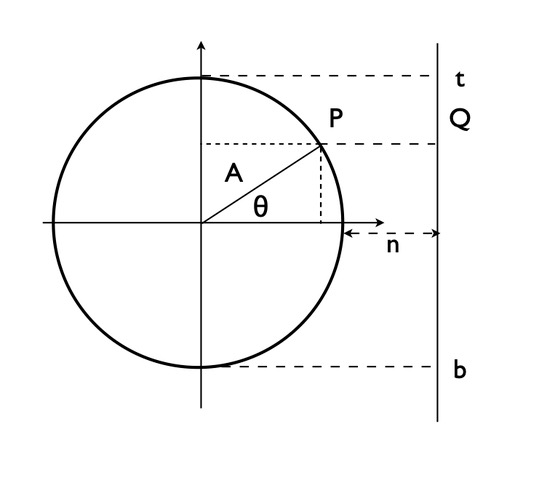
\includegraphics[width=7cm,keepaspectratio]{Figs/harmonic.jpg}
\end{center}
\caption{\small Simple harmonic motion.}
\label{fig:SHM}
\end{figure}
%****************************************************************************************
The points $P$ and $Q$ have coordinates

\[
P=(A\cos\,\omega t, A\sin\,\omega t),\quad Q=(A+n,A\sin\,\omega t),
\]
where $\omega$ is the angular velocity of the particle $P$, with $\omega t=\theta$. The positive real number $n$ is not essential for our purpose.

{\bf {\em Simple harmonic motion}}: an object that moves in such a way that its displacement from equilibrium can be written as $A\sin \,\omega t$ (or $A\cos\,\omega t$, or $A\sin (\omega t+\varphi)$) is said to execute a simple harmonic motion. In our setup, the particle $Q$ executes a simple harmonic motion.

{\bf {\em Amplitude of vibration}}: Maximum displacement (of the object executing the simple harmonic motion) from its equilibrium position. In the situation corresponding to Fig.~\ref{fig:SHM}, the amplitude is $A$.

{\bf {\em Period of simple harmonic motion}}: time needed to complete one oscillation (for the particle $P$ to revolve once around the circle, i.e. time $T$ such that $\theta\equiv 2\pi=\omega T$. In mathematical terms, the period of the function $F(t)=A\sin \omega t$ is the smallest positive real number $T$ such that $F(t+T)=F(t)$. It is indeed $T=\frac{2\pi}{\omega}$ as 

\[
A\sin(\omega[t +\frac{2\pi}{\omega}])=A\sin (\omega t +2\pi)=A\sin \omega t.
\]
{\bf {\em Frequency of simple harmonic motion}}: the inverse of the period $T$, i.e. \break $f=\frac{1}{T}=\frac{\omega}{2\pi}$.


All these concepts are illustrated in Fig.~\ref{fig:sinusoid}, which graphs the function
$A\sin \omega t$ as a function of $t$. (Note that by choosing the origin of time appropriately, the graph also describes the functions $A\cos\,\omega t$ and $A\sin (\omega t+\varphi)$).
%**************************************FIGURE 2**************************************
\begin{figure}[ht]
\begin{center}
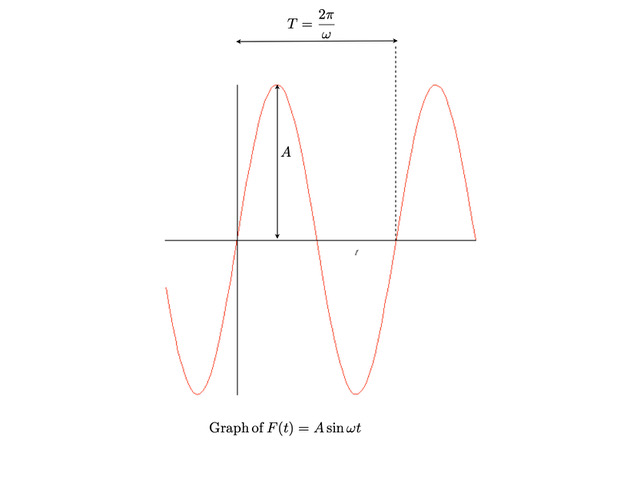
\includegraphics[width=12.7cm,keepaspectratio]{Figs/sinusoid.jpg}
\end{center}
\caption{\small Amplitude and period of $F(t)$.}
\label{fig:sinusoid}
\end{figure}
%****************************************************************************************


\subsection{Orthogonal functions}
Consider two real-valued functions of a real variable, $f_1$ and $f_2$, defined
on the interval $[a,b]$. Introduce the inner product of $f_1$ and $f_2$
on $[a,b]$ as,
\[
(f_1,f_2) \equiv \int_a^b f_1(x)\,f_2(x)\,dx.
\]
\begin{example}
\normalfont
Take $f_1(x)=x,\,f_2(x)=x^2,\,[a,b]=[0,1]$, then
\[
(f_1,f_2)=\int_0^1\,x^3 \,dx = \frac{1}{4}[x^4]_0^1=\frac{1}{4}.
\]
\end{example}
\begin{example}
\normalfont
Take $f_1(x)=x^2,\,f_2(x)=x^3,\,[a,b]=[-1,1]$, then
\[
(f_1,f_2)=\int_{-1}^1\, x^5 \,dx = \frac{1}{6}[x^6]_{-1}^1=0.
\]
\end{example}

In the last example, $(f_1,f_2)=0$ on $[-1,1]$ and one says that $f_1$ and
$f_2$ are orthogonal  on $[-1,1]$.

More generally, the set 
\begin{equation} \label{ortho}
\{\,\cos \frac{\pi k}{p}x\,\}_{k \in \mathbb{N}}\,\cup\,\{\,\sin \frac{\pi k}{p}x\,\}_{k \in \mathbb{N}}
\end{equation}
is an orthogonal set on $(-p,p)$, that is, given {\em non-zero}
integer numbers $m$ and $n$,
\begin{align}
&\int_{-p}^p\cos \frac{m\pi}{p}x\,\cos \frac{n\pi}{p}x\,dx=
\left \{ \begin{array}{l}
0\qquad {\rm for}\,\,m,n > 0, m \neq n\\
p \qquad {\rm for}\,\,m=n,\end{array} \right. \label{coscos}\\ 
&\int_{-p}^p\sin \frac{m\pi}{p}x\,\sin \frac{n\pi}{p}x\,dx=
\left \{ \begin{array}{l}
0\qquad
{\rm for}\,\,m,n > 0, m \neq n\\
p \qquad {\rm for}\,\,m=n,\end{array} \right. \label{sinsin}
\end{align}
while
\begin{equation}
\int_{-p}^p \sin \frac{m\pi}{p}x\,\cos \frac{n\pi}{p}x\,dx=0
\label{sincos}
\end{equation}
 for\,\,$m,n > 0, m \neq n$ as well as for $m=n$. Moreover,
\begin{align}
&\int_{-p}^p 1 \cdot \cos \frac{m\pi}{p}x\,dx=0\qquad
{\rm for}\,\,m> 0,  \label{1cos}\\
&\int_{-p}^p 1 \cdot \sin \frac{m\pi}{p}x\,dx=0\qquad
{\rm for}\,\,m> 0.\label{1sin}
\end{align}
These results are proven by explicit integration, using the well-known
trigonometric identities 
\begin{align*}
\sin(a\pm b)&=\sin a \cos b \pm \sin b \cos a,\\
\cos(a\pm b)&=\cos a \cos b \mp \sin a \sin b.
\end{align*}

For $p=\pi$, one obtains the following important relations
\begin{Framed}
\begin{eqnarray*}
&&\frac{1}{2\pi} \int_{-\pi}^{\pi} \sin mx\,\cos nx \,dx =0\qquad {\rm for}
\,\,m,n \in \mathbb{Z},\\
&&\frac{1}{2\pi} \int_{-\pi}^{\pi} \sin mx\,\sin nx \,dx=\left \{
\begin{array}{l}
0\,\,{\rm if }\,\,m \neq n,\\
\half \,\,{\rm if }\,\,m =n\neq 0,\\
0 \,\,{\rm if }\,\,m =n=0, \end{array} \right.\\
&&\frac{1}{2\pi} \int_{-\pi}^{\pi} \cos mx\,\cos nx \,dx=\left \{
\begin{array}{l}
0\,\,{\rm if }\,\,m \neq n,\\
\half \,\,{\rm if }\,\,m =n\neq 0,\\
1 \,\,{\rm if }\,\,m =n=0. \end{array} \right.
\end{eqnarray*}
\end{Framed}
%%%%%%%%%%%%%%%%%%%%%%%%%%%%%%%%%%%%%%%%
%%%%%%%%%%%%%%%%%%%%%%%%%%%%%%%%%%%%%%%%

\section{Fourier Series}
\setcounter{equation}{0}
\subsection{Definition}
The aim is to represent functions $f(x)$ of period $2p$ in terms of a sum of the constant function 1 and the trigonometric functions in the set \eqref{ortho}, which are all of period $2p$. Starting with $f(x)$ defined on $(-p,p)$, the trigonometric series is of the form
%\footnote{For a nice introduction to Fourier series and their applications,
%read Boas, {\em Mathematical Methods in the Physical Sciences}, Chapter 7.}
\begin{equation} \label{Fourierexp}
\frac{a_0}{2}+\sum_{n=1}^{\infty} [\,a_n\cos \frac{n\pi}{p}x+
b_n\sin \frac{n\pi}{p}x\,],
\end{equation}
with the coefficients being the constants, 
\begin{align}
a_0&=\frac{1}{p}\int_{-p}^p f(x)\,dx\label{a0}\\
a_n&=\frac{1}{p}\int_{-p}^p f(x)\,\cos \frac{n\pi}{p}x\,dx\label{an}\\
b_n&=\frac{1}{p}\int_{-p}^p f(x)\,\sin \frac{n\pi}{p}x\,dx.\label{bn}
\end{align}
The above formulas are often called {\em Euler formulas}.
Note that the coefficient of the constant function 1 is labelled $a_0/2$ rather
than $a_0$; this is for convenience so that the formula for $a_n$ reduces 
to $a_0$ for $n=0$. \\

If the coefficients are such that the series \eqref{Fourierexp} converges, then its sum will be a function of period $2p$. 

\begin{Framed}
\begin{definition}
\normalfont Suppose that $f(x)$ is a given function of period $2p$, which can be represented by a series of the form \eqref{Fourierexp}, and that this series converges and that its sum is $f(x)$. Then, one writes
\begin{equation}
 \label{Fourierexp2}
f(x)=\frac{a_0}{2}+\sum_{n=1}^{\infty} [\,a_n\cos \frac{n\pi}{p}x+
b_n\sin \frac{n\pi}{p}x\,],
\end{equation}
and calls \eqref{Fourierexp2} the  Fourier series of $f(x)$.
\end{definition}
\end{Framed}
In this case, the constants $a_0, a_n, b_n$ for $n>0$ are called the {\em Fourier coefficients} of $f(x)$.

%%%%%%%%%%%%%%%
\subsection{Determination of Fourier coefficients}
Assume that the function $f(x)$ is integrable on $(-p,p)$, and that it is 
equal to its Fourier series, as in \eqref{Fourierexp2}. Also assume that
the series \eqref{Fourierexp2} multiplied by $\cos \frac{m\pi}{p}x$ or
$\sin \frac{m\pi}{p}x$ converges (this is to allow term by term integration of the
series). The  Fourier coefficients \,$a_0,a_n,b_n$ are determined as follows.

$\bullet$ Multiply \eqref{Fourierexp2} by the number 1 and integrate both 
sides between $-p$ and $p$:
\begin{align*}
& \int_{-p}^p  f(x) \cdot  1 \,dx=\\
 &\int_{-p}^p   \{ \, \frac{a_0}{2} \cdot 1 +
\sum_{n=1}^{\infty}[\,a_n \cos \frac{n\pi}{p}x+b_n \sin \frac{n\pi}{p}x\,]
\, \cdot 1 \}\, dx,
\end{align*}
which, after use of \eqref{1cos} and \eqref{1sin}, yields
\[
\int_{-p}^p f(x)\,dx = 2p \frac{a_0}{2}=p\,a_0.
\]

$\bullet$ Multiply \eqref{Fourierexp2} by $\cos \frac{m\pi}{p}x$ where 
$m \neq 0$, and integrate both sides between $-p$ and $p$:
\begin{align*}
& \int_{-p}^p  f(x) \cdot  \cos \frac{m\pi}{p}x \,dx=\\
& \int_{-p}^p \{ \frac{a_0}{2} \cdot \cos \frac{m\pi}{p}x  
 +\sum_{n=1}^{\infty}[\,a_n \cos \frac{n\pi}{p}x+b_n \sin \frac{n\pi}{p}x\,]
\, \cdot \cos \frac{m\pi}{p}x \,\} dx  ,
\end{align*}
which gives, after use of \eqref{1cos}, \eqref{coscos} and \eqref{sincos},
\[
\int_{-p}^p f(x) \cos \frac{m\pi}{p}x\, dx=p\,a_m.
\]
$\bullet$ Multiply \eqref{Fourierexp2} by $\sin \frac{m\pi}{p}x$ where 
$m \neq 0$, and integrate both sides between $-p$ and $p$:
\begin{align*}
 &\int_{-p}^p  f(x) \cdot \sin \frac{m\pi}{p}x \,dx=\\
 &\int_{-p}^p  \{ \, \frac{a_0}{2} \cdot \sin \frac{m\pi}{p}x +
\sum_{n=1}^{\infty}[\,a_n \cos \frac{n\pi}{p}x+b_n \sin \frac{n\pi}{p}x\,]
\cdot \sin \frac{m\pi}{p}x \,\} dx ,
\end{align*}
which gives, after use of \eqref{1sin}, \eqref{sincos} and \eqref{sinsin},
\[
\int_{-p}^p f(x) \sin \frac{m\pi}{p}x\, dx=p\,b_m.
\]
\vskip 1cm

\begin{example}
\normalfont
 Expand 
\begin{equation} \label{example}
f(x)=\left \{ \begin{array}{l}
              0 \,\,{\rm for }\,\,-\pi < x < 0,\\
              \pi-x \,\, {\rm for}\,\, 0 \le x < \pi\end{array} \right.
\end{equation}
in a Fourier series. The graph of $f(x)$ is given in Fig.~\ref{fig:fourier1}.\\
%----------------------------------------- Figure 3 --------------------
\begin{figure}[ht]
\begin{center}
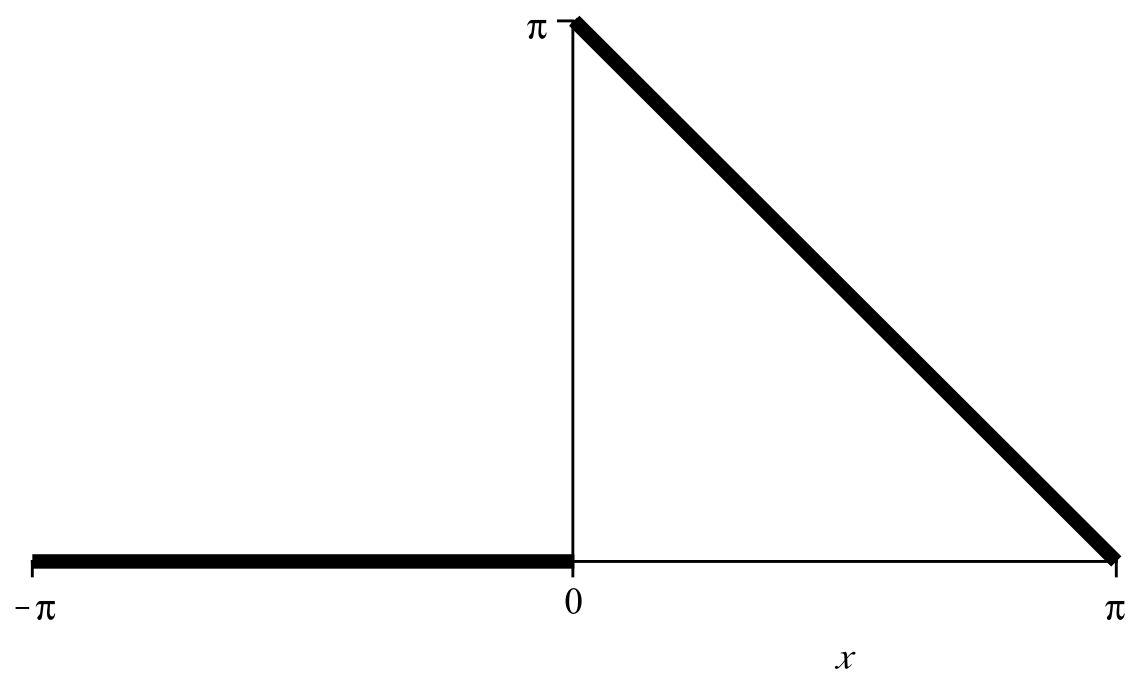
\includegraphics[width=4.9cm,keepaspectratio]{Figs/saw1.jpg}
\end{center}
\caption{\small Graph of $f$ on $(-\pi,\pi)$.}
\label{fig:fourier1}
\end{figure}
%--------------------------------------------------------------------------
\underline{Solution}:
Here, $p=\pi$ and application of \eqref{a0} yields
\[
a_0=\frac{1}{\pi}\int_{-\pi}^{\pi} f(x)\,dx=\frac{1}{\pi}\int_{-\pi}^{0}0\,dx
+\frac{1}{\pi}\int_0^{\pi}(\pi -x)\,dx =\frac{\pi}{2}.
\]
On the other hand, application of \eqref{an} yields  
\begin{align*}
&a_n=\frac{1}{\pi}\int_{-\pi}^{\pi} f(x)\,\cos nx \,dx=\\
&\frac{1}{\pi}\int_0^{\pi}(\pi -x)\,\cos nx \,dx=\frac{1}{n\pi} 
[-\frac{\cos nx}{n}]_0^{\pi} = -\frac{1}{n^2\pi} [ (-1)^n-1],
\end{align*}
where integration by parts has been used (set $u=x, dv= \cos nx dx$).
Finally, application of \eqref{bn} yields 
\begin{align*}
b_n&=\frac{1}{\pi}\int_{-\pi}^{\pi} f(x)\,\sin nx \,dx=
\frac{1}{\pi}\int_0^{\pi}(\pi -x)\,\sin nx \,dx\\
&=\int_0^{\pi} \sin nx\,dx -\frac{1}{\pi} \int_0^{\pi} x\sin nx \,dx 
\nonumber\\
&=-[\frac{\cos nx}{n}]_0^{\pi} -\frac{1}{\pi}[-\frac{x}{n}\cos nx ]_0^{\pi}
+\frac{1}{n}\int_0^{\pi} \cos nx \,dx\\
&=-\frac{1}{n}[(-1)^n-1]+\frac{1}{n\pi} [ (-1)^n\pi -0]=\frac{1}{n},
\end{align*}
where integration by parts has been used (set $u=x, dv=\sin nx dx$).

So the Fourier expansion of $f(x)$ on the interval $(-\pi, \pi)$ is given
by,
\begin{equation} \label{series}
\frac{\pi}{4} + \sum _{n=1}^{\infty} \{ \frac{1-(-1)^n}{n^2\pi}\cos nx
+ \frac{1}{n} \sin nx \}.
\end{equation}
One can tidy the final expression a bit more, as $1-(-1)^n=0$ when $n$ is even, while  $1-(-1)^n=2$ when $n$ is odd. Therefore, only the terms corresponding to $n$ odd will survive in the cosine series of \eqref{series}. Let us thus set $n=2k-1$, and sum over $k$ rather than $n$. This yields
\begin{equation}  \label{series2}
\frac{\pi}{4} + \sum _{k=1}^{\infty} \{ \frac{2}{(2k-1)^2\pi}\cos (2k-1)x
+ \frac{1}{k} \sin kx \}.
\end{equation}
\end{example}

\vskip 1cm
\begin{example}
\normalfont
The {\em delta function} $\delta(x)$ is defined to be the `function' which is equal to $0$ everywhere except at $x=0$, and which satisfies
\[
\int_a^b \delta(x)\,f(x)\,dx= f(0)
\]
when $0 \in [a,b]$. Note that $\delta(x)$ is not, {\em actually}, a function. It is a {\em distribution}, which is a generalization of the function concept, and it is used extensively in mathematical physics. Let us calculate the Fourier coefficients of $\delta(x)$, considered defined on $(-p,p)$. Using the formulas \eqref{a0}-\eqref{bn}, we get,
\begin{eqnarray*}
a_0&=&\frac{1}{p}\int_{-p}^p \delta(x)\,dx=\frac{1}{p}\\
a_n&=&\frac{1}{p}\int_{-p}^p \delta (x)\,\cos\,\frac{n\pi}{p}x\,dx=\frac{1}{p}\cos 0=\frac{1}{p}\\
b_n&=&\frac{1}{p}\int_{-p}^p\delta(x)\,\sin\,\frac{n\pi}{p}x\,dx=\frac{1}{p}.\sin 0=0.
\end{eqnarray*}
\end{example}
\begin{remark}
\normalfont The calculation of Fourier coefficients is quite tedious, and if you need to calculate such quantities in your future career, you may benefit from developing a Maple code to this effect. An example of such code is posted on the course webpages (see Handouts). You are encouraged to experiment with it.
\end{remark}
%%%%%%%%%
%%%%%%%%%

\subsection{Convergence of a Fourier Series}

\subsubsection{Sequence of Partial Sums}
Fourier series do not always converge, and even if they do converge, they do not necessarily converge to the function that generated them. In order to get insight into convergence, let us consider the sequence of partial sums
 $\{ S_m(x), m\ge 1 \}$ of the Fourier series generated by the function $f(x)$,
where
\[
S_m(x)=\frac{a_0}{2}+\sum_{n=1}^m (a_n \cos \frac{n\pi}{p}x+b_n \sin \frac{n\pi}{p}x ).
\]
If the sequence of partial sums converges to $f(x)$ for some $x \in (-p,p)$, i.e.
if
$$
\boxed{f(x)=\lim _{m\rightarrow \infty} S_m(x)}
$$
then the Fourier series converges to $f(x)$ at that value of $x$ and one writes
\[
f(x)=\frac{a_0}{2}+\sum_{n=1}^\infty (a_n \cos \frac{n\pi}{p}x+b_n \sin \frac{n\pi}{p}x ).
\]

For instance, the $m^{th}$ partial sum corresponding to the Fourier series \eqref{series} is,
\[
S_m(x)= \frac{\pi}{4}+\sum _{n=1}^m \{ \frac{1-(-1)^n}{n^2\pi} \cos nx + 
\frac{1}{n} \sin nx \}.
\]
Observe the plots for  $S_2(x), S_4(x)$ and $S_{14}(x)$ shown in Fig.~\ref{fig:fourier3}, and 
compare with the graph in Fig.~\ref{fig:fourier1}. As $m$ increases, it becomes more and more difficult to distinguish $S_m$ from the graph of $f(x)$, and we can be fairly confident that the Fourier series of $f(x)$ converges to $f(x)$ for all $x \in (-\pi,\pi)$.
%----------------------------------------- Figure 4 --------------------
\begin{figure}[H]
\centering
\begin{tabular}{cc}
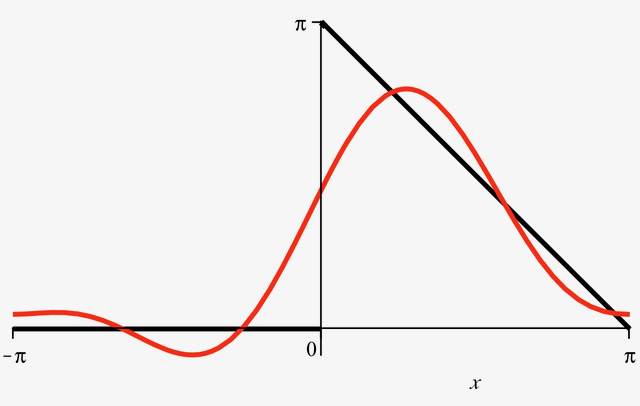
\includegraphics[scale=0.25]{Figs/s2.jpg}~~&~~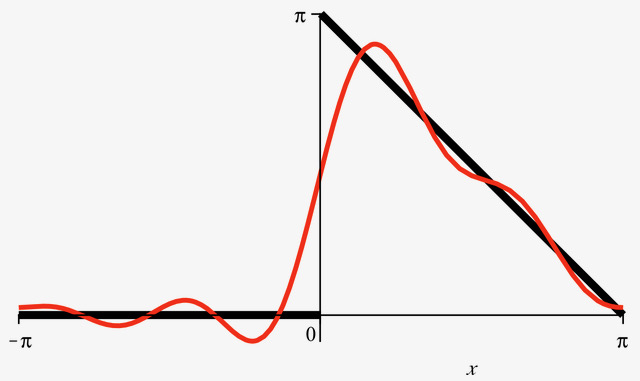
\includegraphics[scale=0.25]{Figs/s4.jpg}\\
$S_2(x)$&$S_4(x)$\\
&\\
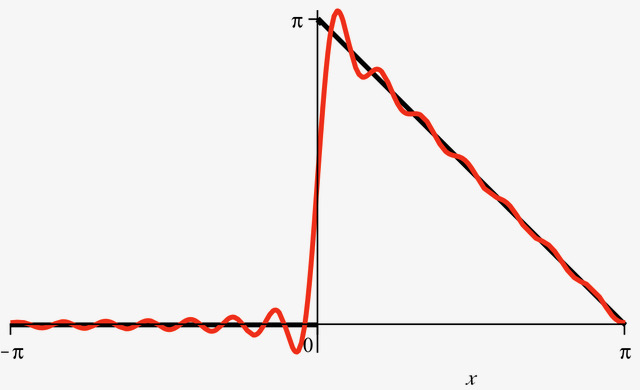
\includegraphics[scale=0.25]{Figs/s14.jpg}~~&~~\\
$S_{14}(x)$&
\end{tabular}
\caption{\small Second, fourth and fourteenth  partial sums of $f$.}
\label{fig:fourier3}
\end{figure}
%--------------------------------------------------------------------------
%%%%%%%%
\subsubsection{Convergence theorem}

\begin{theorem}
\normalfont Let \( f \) and $f'$ be continuous functions, except at a
finite number of points in the interval $(-p,p)$ (i.e. let $f$ and $f'$ be piecewise continuous on $(-p,p)$), and let them only have
finite (jump) discontinuities at these points. Then,

$\bullet$ At a point of continuity $x$, the Fourier series of $f$ on $(-p,p)$
converges to $f(x)$.

\noindent $\bullet$ At a point of discontinuity $x_0$, the Fourier series converges to 
the average
\[
\frac{f(x_{0+})+f(x_{0-})}{2},
\]
where
\begin{eqnarray*}
f(x_{0+})&=& \lim_{h \rightarrow 0}f(x_0+h)\qquad h>0,\\
f(x_{0-})&=& \lim_{h \rightarrow 0}f(x_0-h)\qquad h>0.
\end{eqnarray*}
In other words, it converges to the midpoint of the jump. Moreover, if $f(-p)\neq f(p)$, its Fourier series converges to the average of the endpoints at both ends, as illustrated in Fig.~\ref{fig:cgence} (for $p\equiv \pi$).
\end{theorem}
\begin{proof}
Left as an exercise.
\end{proof}

%----------------------------------------- Figure 5 --------------------
\begin{figure}[H]
\centering
\begin{tabular}{cc}
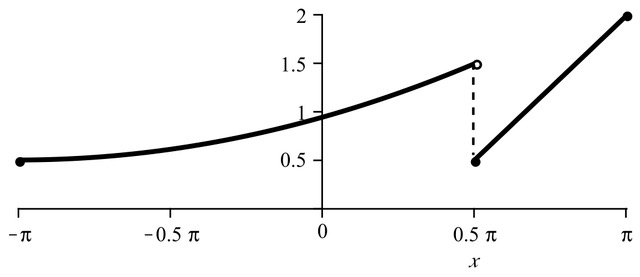
\includegraphics[scale=0.35]{Figs/cgence1.jpg}~~&~~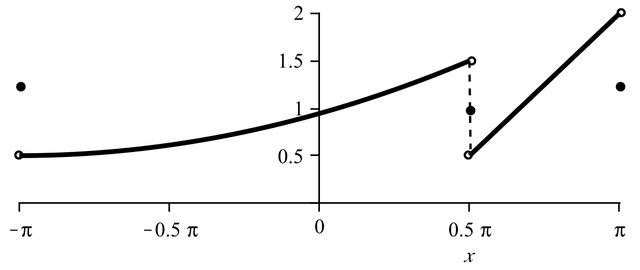
\includegraphics[scale=0.35]{Figs/cgence2.jpg}
\end{tabular}
\caption{\small A piecewise continuous function on $[-\pi,\pi]$ (left) generates a Fourier series converging to the function on the right.}
\label{fig:cgence}
\end{figure}
%----------------------------
In summary,
\begin{Framed}
	If the function $\mathsf{f(x)}$ is piecewise smooth on $\mathsf{x\in(-p, p)}$ then the
	sequence of truncated Fourier series converges as follows:
	\begin{eqnarray*}
	&&\mathsf{\lim_{N\to\infty}S_N(x)} \to \mathsf{ \frac{1}{2}\left(\lim_{y\,\downarrow\, x}f(y) + \lim_{y\,\uparrow\, x}f(y)\right)}\\
	&&= \left\{\begin{array}{l } \mathsf{f(x)} \,\, \textsf{if}\,\, \textsf{f}\, \,\textsf{is continuous
	at}\,\, \textsf{x},\\
	\textsf{average of}\,\, \textsf{f(x)}\,\,\textsf{across jump at a}\\
	\quad \textsf{ discontinuity in}\,\, \textsf{f(x)}
	\end{array}\right.
	\end{eqnarray*}
	($\mathsf{y \downarrow x}$\, \textsf{and}\, $\mathsf{y \uparrow x}$\, \textsf{denote the one-sided
	limits as}\, $\mathsf{y}$ \textsf{approaches}\, $\mathsf{x}$\, \textsf{from above or below respectively.)}
\end{Framed}

\begin{remark}
\textcolor{red}{The above also illustrates how to produce sans serif fonts for both text and formulas (through textsf and mathsf).}
\end{remark}

\section{Miscellaneous}
A few more environments that LaTeXml processes without problems.

The three matrices $\mathsf{M_1, M_2, M_3}$  below are rendered reasonably well in html via LaTeXml.
\[\mathsf{
M_1=
\begin{bmatrix} 
\textsf{a} & \textsf{b} & \textsf{c }\\
d& e & f\\
g & h& i \\
\end{bmatrix},\quad
M_2=
\begin{pmatrix} 
\mathsf{x^2} & \mathsf{\frac{a}{b}} & \textsf{c/b} \\
c & d & e\\
f & g & h \\
\end{pmatrix}},\quad
M_3=
\left[
\begin{array}{c|c}
A & B \\
\hline
C & D
\end{array}
\right].
\]

\end{document}

%%%%%%%%%%%%%%%%%%%%%%%%%%%%%%%
%%%%%%%%%%%%%%%%%%%%%%%%%%%%%%%
